%! suppress = NonBreakingSpace
\documentclass[a4paper,12pt]{article}
\usepackage[english, finnish]{babel}
\usepackage[style=dmyyyy,datesep=.]{datetime2}
\usepackage{setspace}
\usepackage{makecell}
\usepackage{layout}
\usepackage{graphicx}
\usepackage[top=2.5cm,bottom=3cm,left=4cm,right=2cm,includehead]{geometry}
\usepackage{lastpage}
\usepackage{listings}
\usepackage{multirow}
\usepackage{amsmath}
\usepackage{url}
\usepackage{listings}
\usepackage{listings-rust}
\usepackage{tikz}
\usepackage{setspace}
\usepackage{framed}
\usepackage{parskip}
\usepackage{xcolor}
\usepackage{tabularray}
\usepackage{tabularx}
\usepackage[T1]{fontenc}
\usepackage{csquotes}
\usepackage[titles]{tocloft}
\usepackage{fancyhdr}
\usepackage{caption}
\usepackage[square, numbers, semicolon]{natbib}

\bibliographystyle{metro}

\captionsetup{justification=raggedright,singlelinecheck=false}


\renewcommand{\cftdot}{}

\fancyhead{}
\fancyhead[R]{\thepage}
\fancyfoot{}

\renewcommand{\headrule}{}

%\usepackage{helvet}
%\renewcommand{\familydefault}{\sfdefault}
\usepackage{fontspec}
\setmainfont{Arial}


%\usepackage{showframe}
\lstset{language=Rust, style=boxed,
    captionpos=b,
    literate={ö}{{\"o}}1
        {ä}{{\"a}}1
}
\renewcommand{\lstlistingname}{Lähdekoodi}

\definecolor{title}{RGB}{155, 50, 35}


\usepackage{tikz}
\usetikzlibrary{positioning,shapes,shadows,arrows}

\tikzstyle{struct}=[rectangle, draw=black, text centered, anchor=north, text=black, text width=4cm]
\tikzstyle{thread}=[rectangle, draw=black, text centered, anchor=north, text=black, text width=4cm]
\tikzstyle{app}=[rectangle, draw=black, text centered, anchor=north, text=black, text width=3cm]



\newcommand{\architecture}{
\begin{figure}[h!]
\centering
    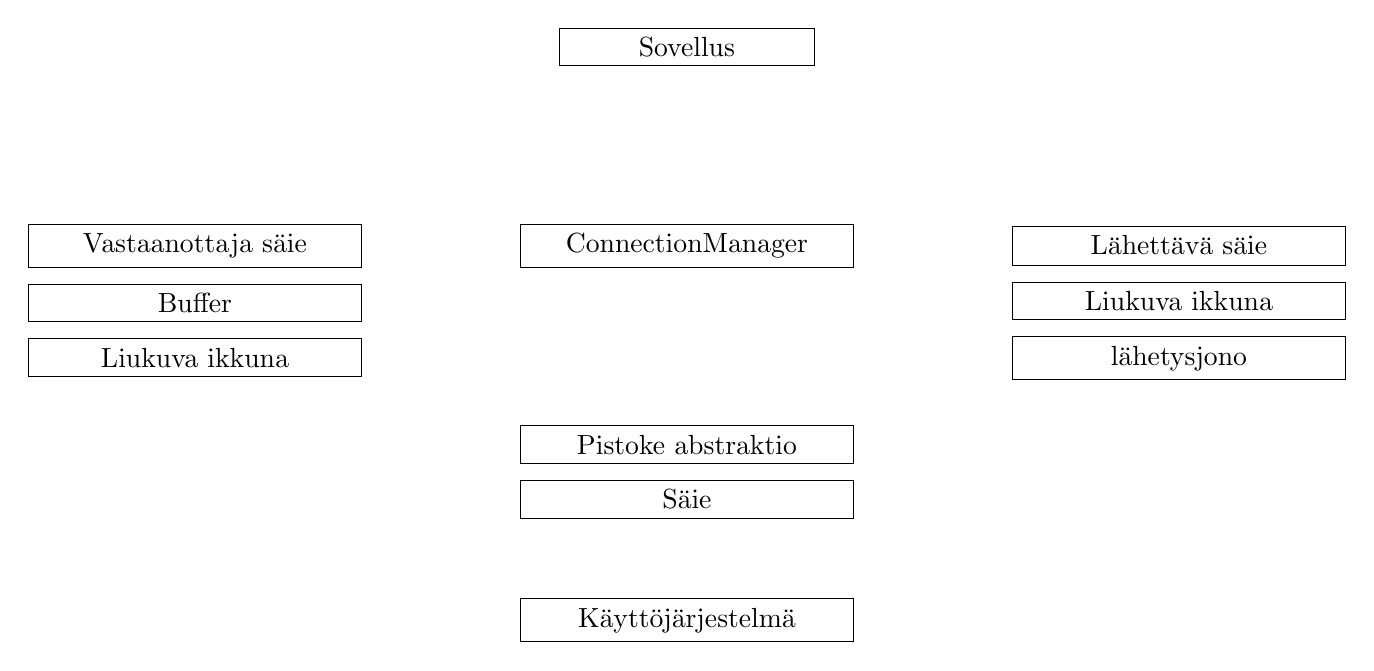
\begin{tikzpicture}[node distance=2cm]
        \node(app)[app]{
            Sovellus
        };
        \node(ConnectionManager)[struct, below=of app] {
            ConnectionManager
        };
       \node(rthread)[thread, left=of ConnectionManager]{
            Vastaanottaja säie
       };
       \node(buffer)[struct, below=0.2cm of rthread] {
            Buffer 
       };
       \node(rwindow)[struct, below=0.2cm of buffer] {
            Liukuva ikkuna 
       };
       \node(tthread)[thread, right=of ConnectionManager]{
            Lähettävä säie
       };
       \node(twindow)[struct, below=0.2cm of tthread] {
            Liukuva ikkuna 
       };
       \node(queue)[struct, below=0.2cm of twindow] {
            lähetysjono
       };
       \node(socket)[struct, below=of ConnectionManager]{
            Pistoke abstraktio
       };
       \node(socketthread)[struct, below=0.2cm of socket]{
            Säie
       };
       \node(os)[struct, below=1cm of socketthread]{
            Käyttöjärjestelmä
       };
    \end{tikzpicture}
    \caption{Arkkitehtuuridiagrammi} \label{fig:arkkitehtuuri}
\end{figure}
}
\usepackage{tikz}
\usetikzlibrary{positioning,shapes,shadows,arrows,quotes,fit}

\tikzstyle{data}=[rectangle, draw=black, text centered, anchor=north, text=black, inner sep=0.5cm]

\tikzstyle{title}=[font=\fontsize{6}{6}\color{black!50}]

\usetikzlibrary{arrows.meta}
\tikzset{>={Latex[scale=1.2]}} 


\newcommand{\slidingWindow}{
\begin{figure}[h!]
\centering
    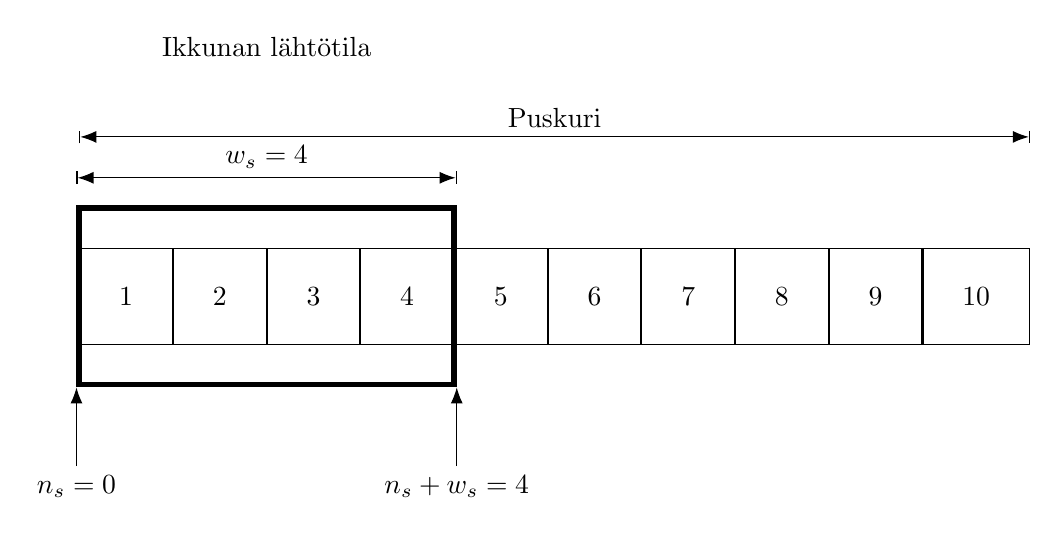
\begin{tikzpicture}[]
        
        \node(data1)[data]{1};
        \foreach \x [remember=\x as \lastx (initially 1)] in {2,...,10}{
            \node(data\x)[data, right=0cm of data\lastx]{\x};
        };
        
        
        \node (window) [draw=black, line width=2pt, inner xsep=0, inner ysep=0.5cm, fit=(data1) (data2) (data3) (data4) ] {};
        
        \node (windowStart)[below=of window.south west]{$n_s = 0$};
        \draw [->] (windowStart) -- (window.south west);
        
        \node (windowEnd)[below=of window.south east]{$n_s + w_s = 4$};
        \draw [->] (windowEnd) -- (window.south east);
        
        \node (windowDesc) [above=5.0em of window] {Ikkunan lähtötila};

        \draw [|<->|] ([yshift=1em]window.north west) -- node[above] {$w_s = 4$} ([yshift=1em]window.north east);
       
        \draw [|<->|] ([yshift=4.0em]data1.north west) -- node[above] {Puskuri} ([yshift=4.0em]data10.north east);
        
    \end{tikzpicture}
    \\[1cm]
    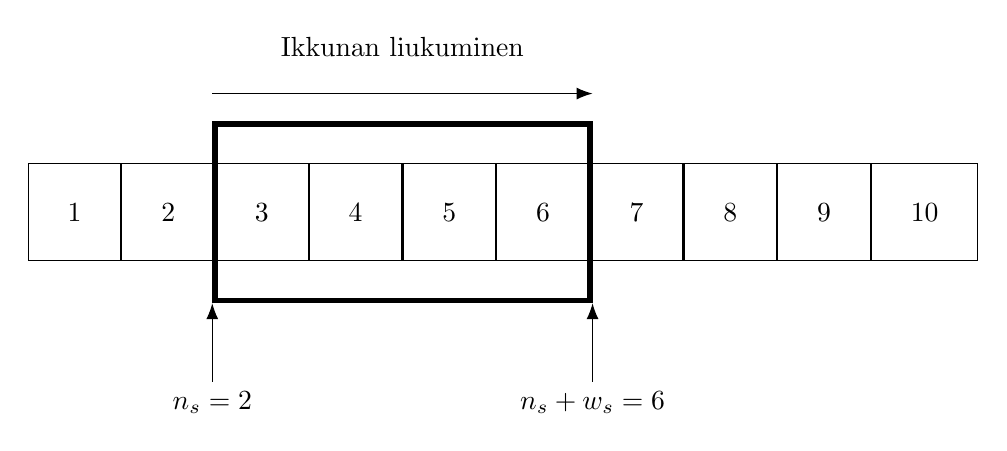
\begin{tikzpicture}[]
    
        \node(data1)[data]{1};
        \foreach \x [remember=\x as \lastx (initially 1)] in {2,...,10}{
            \node(data\x)[data, right=0cm of data\lastx]{\x};
        };
        
        
        \node (window) [draw=black, line width=2pt, inner xsep=0, inner ysep=0.5cm, fit=(data3) (data4) (data5) (data6) ] {};
        
        
        \node (windowDesc) [above=2.0em of window] {Ikkunan liukuminen};

        \node (windowStart)[below=of window.south west]{$n_s = 2$};
        \draw [->] (windowStart) -- (window.south west);
        
        \node (windowEnd)[below=of window.south east]{$n_s + w_s = 6$};
        \draw [->] (windowEnd) -- (window.south east);
        
        \draw [->] ([yshift=1em]window.north west) -- ([yshift=1em]window.north east);
        
    \end{tikzpicture}
    \caption{Liukuvan ikkunan toiminta} \label{fig:sliding_window}
\end{figure}
}


\onehalfspacing


\usepackage[linktoc=all]{hyperref}
\hypersetup{
    colorlinks,
    citecolor=black,
    filecolor=black,
    linkcolor=black,
    urlcolor=black
}


\renewcommand{\title}{Luotettavan tietoliikenneprotokollan \newline suunnittelu ja toteutus Rustilla}
\newcommand{\englishTitle}{Design and implementation of a reliable communication protocol in Rust}

\author{Joonas Kajava}
\date{\today}

\newcommand{\me}{Joonas Kajava}

\newcommand{\appendixCount}{0}

\newcommand{\pageCount}{ \pageref{LastPage}}

\newcommand*\sepline{
    \begin{center}
        \rule[1ex]{\textwidth}{.5pt}
    \end{center}}


\begin{document}
    \begin{titlepage}
    
        \pagestyle{empty}
        
        \includegraphics[width=9.1cm,height=9.1cm]{images/metropolia}\par\vspace{2cm}
        {\Large \me}\par \vspace{1cm}

        {\Huge \textcolor{title}{\title}}\par \vspace{1cm}

        \vfill

        Metropolia Ammattikorkeakoulu\par
        Insinööri (AMK)\par
        Tieto ja viestintätekniikka\par
        Insinöörityö\par
        \today

        \newpage



        \section*{Tiivistelmä}

\setlength{\tabcolsep}{0cm}
        \begin{tabular} {p{5cm} p{10cm}}
            Tekijä:               & \me                                            \\
            Otsikko:              & \title                                         \\
            Sivumäärä:            & \pageCount{} sivua                             \\
            Aika:                 & \today                                         \\
            \\
            Tutkinto: & Insinööri (AMK) \\
            Tutkinto-ohjelma: & Tieto- ja viestintätekniikka \\
            Ammatillinen pääaine: & Pelisovellukset \\
            Ohjaajat: & Lehtori Miikka Mäki-Uuro\\
        \end{tabular}
        \sepline
        \begin{singlespace}
        
        Tässä insinöörityössä esitetään luotettavan tietoliikenneprotokollan suunnittelu ja toteutus, minkä nimeksi tuli RRTP-protokolla. Protokollaa varten tehtiin ohjelmakirjasto Rust-kielelle, mistä lopputuloksena syntyi RRTP-protokollan toteuttava ohjelmakirjasto. Se yhdistää liukuvan ikkunan ja muita tekniikoita luotettavan yhteyden muodostamiseen. \par

        Protokollan toimivuus testattiin demosovelluksella, joka kehitettiin tässä työssä käyttämällä Tauri-ohjelmistokehystä. Tauri-ohjelmistokehys hoitaa käyttöliittymän piirtämisen. Sovellus hyödyntää RRTP-ohjelmakirjastoa yhteyden muodostamiseen ja tiedon välittämiseen kahden tietokoneen välillä. \par

        Kehityksen aikana toteutettiin suorituskykyanalyysejä, joissa vertailtiin tietorakenteiden nopeuksia protokollan käyttötarkoituksissa. Analyysin perusteella todettiin, että LinkedList-tietorakenne ei ole sopiva tähän projektiin. Toteutukseen valittiin Vec-tietorakenne, jonka suorituskyky oli erinomainen ja joka sopii parhaiten projektin käyttötarkoituksiin.\par

        Lopuksi pohdittiin työtapoja ja työkaluja, joita käytettiin kehityksessä. Työssä käytettiin Git-versionhallintaa ja kehitysympäristö koostui Windows-tietokoneesta sekä RustRoverista, joka on Rust-kieleen erikoistunut ohjelmointiympäristö. 
        
        \end{singlespace}
        
        \par
        \begin{tabular} {p{5cm} l}
            Avainsanat: & Rust, UDP, suorituskyky, liukuva ikkuna, protokolla \\
       \end{tabular} 
        \sepline
        Tämän opinnäytetyön alkuperä on tarkastettu Turnitin Originality Check -ohjelmalla.
        
        \newpage
        
        \section*{Abstract}

        \begin{tabular} {p{5cm} p{10cm}}
            Author:               & \me                                            \\
            Title:                & \englishTitle                                  \\
            Number of Pages:      & \pageCount{} pages                             \\
            Date:                 & {\selectlanguage{english}\today}                                         \\
            \\
            Degree:               & Bachelor of Engineering                        \\
            Degree Program:    & Information and Communication Technology       \\
            Professional Major:   & Game Applications                              \\
            Supervisors:          & Senior Lecturer Miikka Mäki-Uuro            \\
        \end{tabular}
        \sepline

\begin{singlespace}
    

        This Bachelor's thesis goes through design and implementation of a reliable communication protocol. RRTP-protocol was given for this communication protocol. Library for Rust programming language was created for the protocol and its implementation will be showcased in the thesis. End product was a library that implements RRTP-protocol, which combines sliding window and other techniques for a reliable connection.\par

        Robustness of the protocol is tested using a demo application that was also developed in this thesis. The application was created using Tauri-framework. Tauri-framework handles drawing the user interface. Demo application utilizes RRTP-library to handle connection and data transfer between two computers. \par

        During development performance analysis was performed for data structures used in the protocol. Analysis indicated that LinkedList data structure is not suitable for this project, while Vec data structure is more appropriate for this project.
        \par

        The thesis concludes with a reflection section that discusses development practices and tools used in this thesis. Git was used as the version control system and development environment consisted of Windows machine with RustRover.

\end{singlespace}

        \begin{tabular} {p{5cm} l}
            Keywords: & Rust, UDP, performance, sliding window, protocol \\
        \end{tabular}
        \newpage

        \tableofcontents
        \newpage
        
        \addtocontents{toc}{\protect\contentsline{section}{Lyhenteet}{}{}}
        
        \section*{Lyhenteet}
        \begin{tblr}{
        colspec = {l X}, rowsep = 1ex
        }
            ACK: & \textit{Acknowledgement}. Vastaanottajan kuittaus saapuneesta paketista. \\
            API: & \textit{Application Programming Interface}. Komponenttien välinen ohjelmointirajapinta. \\
            ARQ: & \textit{Automatic Repeat Request}. Automaattinen uudelleenlähetys.\\
            DI:  & \textit{Dependency Injection}. Riippuvuuksien injektointi, jonka avulla tarvittavat riippuvuudet on saatavilla tietyissä aliohjelmissa. \\
            IP:  & \textit{Internet Protocol}. IP-pakettien toimituksesta huolehtiva protokolla. \\
            IPC: & \textit{Inter-Process Communication}. Prosessien välinen kommunikaatio. \\
            MIME: & \textit{Multipurpose Internet Mail Extensions}. MIME-tyyppi kertoo tiedostomuodon standardin mukaisella tavalla. \\
            NACK: & \textit{Negative Acknowledgement}. Negatiivinen vastaanottajan kuittaus. \\
            NIC: & \textit{Network Interface Controller}. Verkkosovitin, jonka tehtävä on muodostaa yhteys lähiverkkoon. \\
            RPC: & \textit{Remote Procedure Call}. Etäproseduurikutsu, jonka avulla asiakasohjelma voi lähettää kutsuviestin palvelinohjelmalle. \\
            TCP: & \textit{Transmission Control Protocol}. Tietoliikenneprotokolla, joka muodostaa jatkuvan yhteyden tietokoneiden välille. \\
            UDP: & \textit{User Datagram Protocol}. Yksinkertainen tietoliikenneprotokolla, joka ei tarjoa virheenkorjausta.\\
        \end{tblr}
        \newpage


    \end{titlepage}

\pagestyle{fancy}

\renewcommand{\arraystretch}{1.5}
    \section{Johdanto}\label{sec:johdanto}
    Tässä työssä suunniteltiin ja toteutettiin tietoliikenneprotokolla Rust-kielelle. Tietoliikenneprotokolla käyttää UDP-protokollaa pohjana ja laajentaa sitä uusilla ominaisuuksilla. UDP on yksinkertainen tietoliikenneprotokolla, joka ei tarjoa pakettien järjestämistä tai kattavaa virheenkorjausta. Tarkoitus on luoda pohja yrityksille ja kehittäjille tietoliikenneprotokollan toteutukseen.
    Työ on luonteeltaan tutkiva ja ohjeistava, joka selventää reaaliaikaisien sovelluksien toteutusta.\par

    Protokollaa varten tehtiin RRTP-ohjelmistokirjasto käyttäen Rust-ohjelmointikieltä, joka soveltuu erinomaisesti järjestelmäohjelmointiin. Rust-kieli mahdollistaa laitteiston matalan tason hallinnan
    samaan tapaan kuin C-ohjelmointikieli. Iso etu Rust-kielessä on, että se käyttää automaattista muistinhallintaa, joka ei käytä roskankerääjää, vaan muistin vapautus tapahtuu omistus- ja lainausjärjestelmän sääntöjen mukaisesti.
    Nämä säännöt takaavat Rust-kielen muistiturvallisuuden, joka on todella tärkeää ohjelman toimivuuden kannalta. 
    Rust-kieli tarjoaa myös monia moderneja kieliominaisuuksia kuten tyyppipäättely (engl. type inference), hahmonsovitus (engl. pattern matching) ja piirteet (engl. traits) \cite{rust-book}.

    Johdannon jälkeen siirrytään käsittelemään RRTP-protokollan toteuttavan kirjaston toimintaa. RRTP-kirjasto on neljään osaan jaettu kokonaisuus, joka käyttää säikeitä ja kanavia sisäiseen tiedon siirtoon. Kirjaston avulla ohjelmat, kuten tässä työssä kehitetty demosovellus pystyvät kommunikoimaan viestien ja tiedostojen avulla. 
    Toteutuksen läpikäynti alkaa paketin vakioiden ja rakenteen määrityksellä, jonka jälkeen siirrytään käsittelemään kirjaston arkkitehtuuria. \par

    Luotettavuus tässä tietoliikenneprotokollassa tulee liukuvasta ikkunasta. Se sallii pakettien lähettämisen ja vastaanottamisen epämääräisessä järjestyksessä sekä takaa viestien perille pääsyn aikakatkaisun avulla. Työssä liukuvan ikkunan toiminta esitetään lähettäjän ja vastaanottajan näkökulmista, jossa toiminta havainnollistetaan diagrammien ja koodin avulla. Tämän jälkeen keskustellaan tarkemmin valikoiva toisto ARQ-protokollasta. \par

    Viestien käsittelyssä esitetään eri tietomuodot, joita voidaan käyttää tiedonsiirrossa. Tietomuotojen määritys on tärkeää tiedonsiirrossa, sillä vastaanottajan ja lähettäjän täytyy olla yhteisymmärryksessä niistä. Demosovelluksessa tiedonsiirto tapahtuu käyttäen binäärimuotoa, mutta skeemapohjaisen tiedon käyttäminen on mahdollista. Skeemapohjaisen tiedon ja binääritiedon erot esitetään esimerkkien avulla.\par

    Viimeisenä RRTP-protokollasta esitetään virheenkorjaus, johon kuuluu 16-bittinen tarkistussumma. Sen sijoitus paketissa havainnollistetaan taulukon ja koodin avulla. Lopuksi tarkistussumman muodostus esitetään esimerkkikoodin avulla.\par

    RRTP-kirjastoa varten toteutettiin myös demosovellus, joka tarjoaa 
    toiminnot viestien ja tiedostojen lähettämistä varten. Demosovelluksesta esitetään sen riippuvuudet eri kirjastoihin sekä Rust-prosessin ja 
    käyttöliittymän välisen kommunikaation. \par

    Tämän työn tavoitteena oli tutkia tietoliikenneprotokollien toimintaa ja niiden toteutusta. On usein kannattavaa kehittää sovelluksen tarpeisiin mukautettu protokolla, mikäli kaistanleveys ja vasteaika merkitsee huomattavasti.

   \section{RRTP-protokolla}\label{sec:protocol}
    TCP- ja UDP-protokollat ovat kaksi yleisintä TCP/IP-protokollaa. TCP-protokolla on jatkuvan yhteyden muodostava tietoliikenneprotokolla, jota käytetään usein vakaata ja luotettavaa yhteyttä vaativissa palveluissa, kun taas UDP on usein paras reaaliaikaisia sovelluksia varten. Tämä johtuu siitä, että TCP-paketin mukana liikkuu paljon varattuja tavuja, joita ei käytetä ollenkaan.\par
    
    UDP:n etu reaaliaikaisessa kommunikaatiossa on, että se on kevyt ja nopea. Se ei kuitenkaan tarjoa kattavaa virheenkorjausta, järjestystä tai ruuhkanhallintamekanismeja. Tarkistussumma on ainut virheentarkistus, minkä UDP tarjoaa. Se ei kuitenkaan yksin riitä vakaaseen yhteyteen, vaan lisäksi täytyy huomioida pakettien järjestys. Tämän takia liukuva ikkuna ja automaattinen uudelleenlähetys(AQR) ovat tärkeitä tekniikoita kommunikaation luotettavuudessa, sillä niiden avulla paketit voivat liikkua verkon yli epämääräisessä järjestyksessä. Pakettien uudelleen järjestäminen vastaanottaessa vaatii järjestysnumeron. UDP sisältää
    lähettäjän ja vastaanottajan portit, datan koon, tarkistussumman ja datan.
    [\citenum{KumarSurveyUDP}.]
    \par
   
    Tässä luvussa esitetään RRTP-protokollan toteutus, joka on reaaliaikaiseen kommunikointiin erikoistunut tietoliikenneprotokolla.\par

    Protokollan paketti sisältää ohjausbittejä, jotka ilmaisevat tärkeää tietoa paketista. Näiden bittien avulla vastaanottaja tietää, milloin viimeinen paketti on saapunut perille ja lähettäjä saa tiedon kuittauksesta. 
    Liukuvaa ikkunaa hyödynnetään paketin järjestämiseen ja samanaikaiseen lähettämiseen.
    Vastaanottaja ja lähettäjä voivat välittää paketteja keskenään järjestyksestä riippumatta, sillä ikkunan puskuri järjestää paketit niiden järjestysnumeron mukaan.

    \subsection{Paketti}\label{sec:paketti}
    Paketti, joka on havainnollistettu taulukossa \ref{tab:packet}, perustuu kevyesti TCP:hen ja on rakennettu käyttäen UDP:ta pohjana. Paketin rakenne on minimaalinen ja yksinkertainen, mikä sisältää tarvittavat kentät luotettavaan yhteyteen. Nämä kentät ovat järjestysnumero, ohjausbitit ja kentät datan hallintaa varten. Pakettiin sisältyy yksi tavun kokoinen varattu kenttä, jota voidaan käyttää tulevaisuudessa. 6 ohjausbittiä ei ole käytössä, joita voidaan käyttää myöhemmin uusiin ominaisuuksiin.

    \subsubsection*{Vakiot}
    Taulukkoon \ref{tab:vakiot} on koostettu ne vakiot, jotka ovat tärkeitä protokollan toiminnan kannalta. Vastaanottajalla ja lähettäjällä täytyy olla samat vakiot käytössä, jotta pakettien muodostaminen ja lukeminen onnistuu. Eroavaisuudet näissä vakioissa vastaanottajan ja lähettäjän välillä voivat tarkoittaa, että vastaanottaja aloittaa datan lukemisen väärästä kohdasta.

    \begin{table}[h!]
        \centering
        \caption{Vakiot ja niiden arvot.}
        \label{tab:vakiot}
        \begin{tabularx}{\textwidth}{|X|r|r|r|}
        \hline
            \textbf{Vakion nimi}          & \textbf{Lyhenne} & \textbf{Arvo} & \textbf{Yksikkö} \\ \hline
            MAX\_DATA\_SIZE      & $D_s$   & 128  & Tavu    \\ \hline
            SEQ\_NUM\_SIZE       & $S_s$   & 4    & Tavu    \\ \hline
            CONTROL\_BITS\_SIZE  & $C_s$   & 1    & Tavu    \\ \hline
            RESERVED\_SIZE       & $R_s$   & 1    & Tavu    \\ \hline
            DATA\_LENGTH\_SIZE   & $DL_s$  & 1    & Tavu    \\ \hline
            DATA\_OFFSET\_SIZE   & $DO_s$  & 1    & Tavu    \\ \hline
            OPTION\_KIND\_SIZE   & $OK_s$  & 1    & Tavu    \\ \hline
            OPTION\_LENGTH\_SIZE & $OL_s$  & 1    & Tavu    \\ \hline
            OPTION\_DATA\_SIZE   & $OD_s$  & 4    & Tavu    \\ \hline
            MAX\_OPTION\_COUNT   & $MO_c$  & 4    & Määrä \\  \hline
        \end{tabularx}
    \end{table}

    Näiden vakioiden perusteella voidaan laskea tärkeitä muuttujia, jotka on määritelty kaavojen \ref{eq:fmin}-\ref{eq:optionSize} mukaisesti.

    \begin{align}
        \text{MIN\_FRAME\_SIZE} &= F_{min} = S_s + C_s + R_s + DL_s + DO_s \label{eq:fmin} \\
        \text{MAX\_FRAME\_SIZE} &= F_{max} = F_{min} + MO_c(OK_s + OL_s + OD_s) + D_s \label{eq:fmax} \\
        \text{Frame size} &= F_s \\
        \text{Option size} &= O_s = F_s - F_{min} - D_s \label{eq:optionSize}
    \end{align}

    Vakikoiden ja laskettujen muuttujien perusteella voidaan rakentaa paketin kehys, joka on havainnollistettu taulukossa \ref{tab:packet}.
    Kehys määrittelee jokaisen arvon sijainnin ja pituuden paketissa. Näin lähettäjällä ja vastaanottajalla on yhtenäinen ymmärrys paketin rakenteesta.

    \begin{table}[h!]
        \centering
        \caption{Paketin rakenne}
        \label{tab:packet}
        \resizebox{\textwidth}{!}{
            \begin{tabular}{*{33}{|l}|l|}
                \hline
                \multicolumn{2}{|c|}{Offsets} & \multicolumn{8}{|l|}{0} & \multicolumn{8}{|l|}{1} & \multicolumn{8}{|l|}{2}& \multicolumn{8}{|l|}{3} \\ \hline
                Octet & Bit & 0 & 1 & 2 & 3 & 4 & 5 & 6 & 7 & 0 & 1 & 2 & 3 & 4 & 5 & 6 & 7 & 0 & 1 & 2 & 3 & 4 & 5 & 6 & 7 & 0 & 1 & 2 & 3 & 4 & 5 & 6 & 7 \\ \hline
                0 & 0 & \multicolumn{32}{|c|}{Sequence number} \\ \hline
                4 & 32 & RES & RES & RES & RES & RES & RES & EOM & ACK & \multicolumn{8}{|c|}{Reserved} & \multicolumn{8}{|c|}{Data Length}& \multicolumn{8}{|c|}{Data Offset} \\ \hline
                8 & 64 & \multicolumn{32}{|c|}{Options} \\
                ... & ... & \multicolumn{32}{|c|}{} \\ \hline
                \multicolumn{2}{|c|}{Data Offset} & \multicolumn{32}{|c|}{Data} \\
                ... & ... & \multicolumn{32}{|c|}{} \\ \hline
            \end{tabular}
        }
    \end{table}

    Lähdekoodissa \ref{lst:frame} määritetään tietorakenne \textit{Frame}, joka sisältää kaiken paketissa olevan tiedon.
    [u8; MAX\_FRAME\_SIZE]  on taulukkotyyppi, joka koostuu tavuista ja on kooltaan yhtä suuri kuin F\textsubscript{max}, joka on määritelty kaavassa \ref{eq:fmax}.
    data\_length sisältää tiedon pakettiin tallennetun datan koosta, kun taas options\_size sisältää tiedon paketin asetuksien koosta, mitä käytetään datan asettamisen oikeaan paikkaan ja \textit{'Data Offset'} kentän asettamiseen.
    
    Paketti on määritelty seuraavasti:
    \begin{lstlisting}[caption={Paketin rakenne}, label={lst:frame}]
pub struct Frame {
    frame: [u8; MAX_FRAME_SIZE],
    data_length: usize,
    options_size: usize,
}\end{lstlisting}
    
    usize vastaa kohdearkkitehtuurin muistiosoitteen kokoa. 32-bittisessä tietokoneessa usize vastaa 4 tavua ja 64-bittisessä kohteessa 8 tavua \cite[\textit{usize}]{rust-std}.
   
    \subsubsection*{Tietojenkäsittely paketissa}
    Paketti on ohjelman muistissa yhtenä kokonaisena taulukkona, joka koostuu tavuista.
    Taulukko sisältää tietoja 16-bittisessä ja 32-bittisessä muodossa. Nämä tiedot jaetaan tavuihin lähettämistä varten.

    Lähdekoodissa \ref{lst:set_seq_num} järjestysnumero muutetaan laskevaan tavujärjestykseen käyttäen Rust-standardikirjaston to\_be\_bytes()-aliohjelmaa \cite[\textit{u32}]{rust-std}. Tämän jälkeen tulos kopioidaan paketin ensimmäisen 4 tavun tilalle. \par
    
        \begin{lstlisting}[caption={Järjestysnumeron asettaminen pakettiin}, label={lst:set_seq_num}]
pub fn set_sequence_number(&mut self, sequence_number: u32) {
    let net_sequence_number = sequence_number.to_be_bytes();
    self.frame[SEQUENCE_NUMBER_OCTET..4]
    .copy_from_slice(&net_sequence_number);
}\end{lstlisting}


    Oikea tavujärjestys on erittäin tärkeä osa verkon ylitse tehtävää tiedonsiirtoa. Protokollaa käyttävien tietokoneiden täytyy olla yhteisymmärryksessä siitä, mitä tavujärjestystä tiedonsiirrossa käytetään. Laskeva tavujärjestys on yleisin järjestys, joten sitä käytettiin myös tässä protokollassa. \par
    
    Mikäli tavujärjestystä ei oteta huomioon tiedonsiirrossa ja vastaanottajan sekä lähettäjän tietokoneet käyttävät eri tavujärjestystä, lukujen muuntaminen tavutaulukosta primitiiviseksi luvuksi johtaa vääriin tuloksiin     \cite{Adiga2007HowC}.

    \subsubsection*{Ohjausbitit}\label{subsec:control_bits}
    Ohjausbitit ilmaantuvat paketissa yhtenä tavuna, joista jokainen bitti vastaa tiettyä totuusarvoa.

    Taulukon \ref{tab:control_bits} määrittämät ohjausbitit antavat vastaanottajalle tärkeää tietoa paketista. Kuittausbitti ilmoittaa lähettäjälle, että vastaanottaja on saanut paketin onnistuneesti. Päätebitti ilmoittaa vastaanottajalle, että kyseinen paketti on pakettiryhmän viimeinen ja ryhmä on valmis koottavaksi, kun kaikki sitä edeltävät paketit ovat saapuneet. \par
    
    \begin{table}[h!]
        \centering
        \caption{Ohjausbitit ja niiden arvot}
        \label{tab:control_bits}
        \begin{tabularx}{\textwidth}{|X|r|r|}
        \hline
            \textbf{Nimi}     & \textbf{Lyhenne} & \textbf{Binääriarvo} \\         \hline
            Kuittaus & ACK     & 00000001    \\ \hline
            Pääte    & EOM     & 00000010    \\ \hline
        \end{tabularx}
    \end{table}


    Vastaanottaja tarkistaa ohjausbittien olemassaolon bittioperaatiolla lähdekoodin \ref{lst:ack_check} mukaisesti.
    
    \begin{lstlisting}[float, caption={Kuittausbitin tarkistus ohjausbiteistä}, label={lst:ack_check}]
if control_bits & 00000001 == 00000001 {
    // Kuittausbitti löytyy
}\end{lstlisting}

    \subsection{Arkkitehtuuri}\label{sec:arkkitehtuuri}
    RRTP-protokollan toteuttava kirjasto on jaettu neljään osaan. Nämä osat kommunikoivat keskenään kanavien avulla. Kirjaston arkkitehtuuri on havainnollistettu kuvassa \ref{fig:arkkitehtuuri}. 

    Kirjaston ydin on ConnectionManager, joka on vastuussa yhteyksien hallinnasta. Sen tehtävä on
    hoitaa vastaanottavaa säiettä ja lähettävää säiettä. Kun sovellus haluaa käynnistää yhteyden,
    ConnectionManager luo pistokkeen sovelluksen antamaan osoitteeseen.
    Lähetys- ja vastaanottosäikeet käynnistyvät, kun pistokkeen luonti onnistuu. ConnectionManagerin rakenne on määritelty lähdekoodin \ref{lst:connectionmanager} mukaisesti.
    
    \begin{lstlisting}[caption={ConnectionManagerin rakenne}, label={lst:connectionmanager}]
pub struct ConnectionManager {
    listener_thread: Option<thread::JoinHandle<()>>,
    transmitter_thread: Option<thread::JoinHandle<()>>,
    socket: Arc<SocketAbstraction>,
    message_sender: SyncSender<Vec<u8>>,
}\end{lstlisting}

    

    ConnectionManagerilla on omistajuus vastaanottaja- ja lähettäjäsäikeisiin.
    Option<...> määrittelee valinnaisen arvon, joka tarkoittaa, että kyseinen muuttuja ei
    välttämättä sisällä käyttökelpoista arvoa. Tämä vastaa useissa ohjelmointikielissä null-arvoa \cite[luku 6.1]{rust-book}. Näitä kahta muuttujaa käytetään säikeiden sulavaan sulkemiseen, kun ConnectionManager pudotetaan muistista. ConnectionManager toteuttaa Drop-ominaisuuden, joka liittää vastaanottaja-
    ja lähettäjäsäikeet. Näin ohjelma jää odottamaan, että nämä kaksi säiettä sulkeutuvat oikein \cite[\textit{JoinHandle}]{rust-std}.
    
    \architecture
    

    \begin{lstlisting}[caption={Drop-ominaisuuden toteutus ConnectionManagerille}, label={lst:connectionmanager_drop}]
impl Drop for ConnectionManager {
    fn drop(&mut self) {
        if let Some(x) = self.listener_thread.take() {
            x.join().unwrap();
        }
        if let Some(x) = self.transmitter_thread.take() {
            x.join().unwrap();
        }
    }
}\end{lstlisting}



    \subsection{Liukuva ikkuna}\label{sec:liukuva_ikkuna}
    Liukuva ikkuna on tekniikka, joka sallii pakettien lähettämisen ja vastaanottamisen epämääräisessä järjestyksessä. 
    Kirjasto käyttää kahta liukuvaa ikkunaa, jotka on havainnollistettu arkkitehtuuri kuvassa \ref{fig:arkkitehtuuri}. Lähettäjän ja vastaanottajan ikkunat jakavat suurimman osan toiminnallisuuksista Window-toteutuksen kautta, joka on esitetty lähdekoodissa \ref{lst:window}. 

    
\begin{lstlisting}[caption={Ikkunan rakenne}, label={lst:window}]
pub struct Window {
    frame_status: Vec<bool>,
    window_size: u32,
    window_left_edge: u32,
}\end{lstlisting}

frame\_status-kentällä on kaksi tarkoitusta riippuen siitä, onko kyseessä vastaanotto- tai lähetystila. Kummassakin tilanteessa kenttä on aina ikkunan w\textsubscript{s} kokoinen. Vastaanottotilanteessa kenttä pitää kirjaa onnistuneiden pakettien vastaanottamisesta, kun taas lähetystilanteessa kenttä pitää kirjaa paketeista, jotka ovat saapuneet onnistuneesti toiseen tietokoneeseen.\par

window\_size-kenttä on aina w\textsubscript{s} kokoinen. Ikkunan kokoa on mahdollista muuttaa käyttämällä set\_window\_size-aliohjelmaa, joka muuttaa tämän kentän arvoa ja muuttaa frame\_status-taulukon kokoa.\par

window\_left\_edge vastaa muuttujaa n\textsubscript{s}. Vastaanottajan tilanteessa se sisältää pienimmän järjestysnumeron, jota ei ole vastaanotettu, kun taas lähettäjän tilanteessa se sisältää pienimmän järjestysnumeron, joka ei ole vielä saapunut vastaanottajalle. Muuttujan n\textsubscript{s} kasvaminen tarkoittaa ikkunan liukumista eteenpäin, joka on havainnollistettu kuvassa \ref{fig:sliding_window}. 

    \slidingWindow
    
    Tässä ohjelmassa puskurit ovat toteutettu käyttämällä kasa-allokoituja vektoreita. Vec on yleisesti paras tietorakenne tämän tyylisiä operaatioita varten. Vertailu muihin tietorakenteisiin löytyy osiosta \ref{sec:structures}.

\newpage

    \subsubsection*{Ikkunan siirto vastaanottaessa}

    Vastaanottajan ikkuna määritellään lähdekoodin \ref{lst:rwindow} mukaisesti. Se sisältää yleisen Window-toteutuksen ja buffer-kentän, jonka tarkoitus on toimia puskurina, kunnes ikkunan liukuminen aiheuttaa valmiiden pakettien siirtymisen ylempiin kerroksiin. \par
    
\begin{lstlisting}[caption={Vastaanottajan ikkunan rakenne}, label={lst:rwindow}]
pub struct ReceiverWindow {
    inner_window: Window,
    buffer: Vec<Option<Frame>>,
}\end{lstlisting}

    Rust-kielessä ei pysty tekemään perintää samantyylisesti kuin yleisissä olio-ohjelmointikielissä. Tämän takia
    käytetään koostumus-suunnittelutapaa (engl. \textit{Composition}) \cite{Ivicevic202228Rust}.

    Vastaanottava ikkuna pitää muistissa pienimmän järjestysnumeron n\textsubscript{s}, minkä se on vastaanottanut.
    Vastaanottava ikkuna hylkää kaikki paketit, joiden järjestysnumero on ikkunan ulkopuolella n\textsubscript{x} < n\textsubscript{s} tai n\textsubscript{x} > n\textsubscript{s} + w\textsubscript{s}. Jos järjestysnumero on ikkunan sisällä, se hyväksytään ja merkitään vastaanotetuksi. Mikäli n\textsubscript{x} = n\textsubscript{s} + 1, ikkunaa voidaan siirtää eteenpäin.
    Siirto tapahtuu kulkemalla hyväksyttyjen järjestysnumeroiden listaa eteenpäin, kunnes vastaan tulee järjestysnumero, jota ei ole vielä vastaanotettu. Kulkemisen jälkeen tapahtuneiden askelien määrä lisätään muuntujaan n\textsubscript{s}.

    Tässä toteutuksessa n\textsubscript{s} löytyy yleisen ikkunan (lähdekoodi \ref{lst:window}) sisältä kentästä window\_left\_edge.


    \subsubsection*{Vastaanottajan toiminta}
    Datan vastaanottaminen tapahtuu vastaanottajasäikeessä, joka käynnistetään yhteyden muodostamisessa.
    Säie pyörii ikuisessa silmukassa, jossa ensimmäinen operaatio on ikkunan siirto eteenpäin.

    Lähdekoodi \ref{lst:shift_window} esittää ikkunan siirtämistä eteenpäin, jonka tehtävä on kasvattaa n\textsubscript{s}-arvoa ja ilmoittaa ylemmälle kerrokselle siirron määrä.
    frame\_status viittaa onnistuneesti lähetettyihin tai vastaanotettuihin paketteihin.

    \begin{lstlisting}[caption={Ikkunan siirto}, label={lst:shift_window}]
pub fn shift_window(&mut self) -> usize {
    let mut shift_amount = 0usize;
    for e in self.frame_status.iter() {
        if *e {
            shift_amount += 1;
        } else {
            break;
        }
    }
    self.frame_status.drain(0..shift_amount);
    self.window_left_edge += shift_amount as u32;
    shift_amount
}\end{lstlisting}

    Lähdekoodissa \ref{lst:shift_rwindow} data puretaan puskurista ja puskuria siirretään eteenpäin. Tämä operaatio tuottaa
    listan paketeista, jotka ovat saapuneet onnistuneesti ja ovat oikeassa järjestyksessä. Kuva \ref{fig:sliding_window} havainnollistaa puskurin siirron ja siitä syntyvät paketit.
    Lista käsitellään flatten-aliohjelmalla, joka tuottaa listan, missä Option
    on suodatettu pois. Lopuksi puskurin kapasiteettia kutistetaan. Käsitelty lista talletaan ja siirretään käsiteltäväksi ylempiin kerroksiin. \par


    \begin{lstlisting}[caption={Datan purkaminen puskurista}, label={lst:shift_rwindow}]
pub fn shift_window(&mut self) -> Vec<Frame> {
    let shift_amount = self.inner_window.shift_window();
    let shifted_frames = self.buffer.drain(0..shift_amount);
    let result = shifted_frames.into_iter().flatten().collect();
    self.buffer.shrink_to_fit();
    result
}\end{lstlisting}

    Jokainen valmis paketti käsitellään ja niiden sisältö lisätään ylemmän kerroksen puskuriin, minkä jälkeen ohjausbitit luetaan paketista kappaleen \ref{subsec:control_bits} mukaisesti. Vastaanotetusta paketista välitetään tieto ylempiin kerroksiin (kuten sovellukseen), jotka voivat käyttää tätä tietoa esim. latausilmaisimen tekemiseen. \par

    Mikäli paketti on viimeinen viesti, puskuri siirretään uuteen listaan ja välitetään ylemmille kerroksille.

    \subsubsection*{Lähettäjän toiminta}\label{subsec:sender_impl}
    Dataa voidaan lähettää käyttämällä ConnectionManagerista löytyvällä kanavalla. Lähettäjäsäie seuraa tätä kanavaa ja käsittelee sieltä tulevat viestit. \par

    Aluksi viestit leikataan osiin, jossa jokainen osa on kooltaan D\textsubscript{s} tai pienempi. Tämän jälkeen valmis kehys lisätään jonoon, josta se lähetetään käyttäen lähetys säikeen liukuvaa ikkunaa.
 
Lähetyssäie lukee data\_queue-taulukkoa ja aloittaa datan lähettämisen, kun se sisältää kehyksiä. Taulukko käsitellään ja jokaisen kehyksen tilanne luetaan. Jokaisella kehyksellä on kolme mahdollista tilaa: ei lähetetty, lähetetty ja kuitattu. Pakettien lähtötilanne on ei lähetetty. Mikäli taulukon läpikäydessä kohdataan jo aikaisemmin lähetetty kehys, sen lähetysajankohtaa verrataan aikakatkaisu muuttujaan. Aikakatkaisun avulla lähettäjä voi lähettää kehyksen uudelleen, mikäli lähetys ajankohdasta on kulunut tarpeeksi aikaa. Lähetyksen jälkeen kehyksen tila päivitetään lähetetty-tilaan, jonka mukana kulkee tieto lähetysajankohdasta. \par

Lähetyssäie seuraa myös lähdekoodissa \ref{lst:twindow} määritettyä kuittauskanavaa, joka välittää tiedon ACK-paketin saapumisesta. Tieto paketin saapumisesta tulee kuvan \ref{fig:arkkitehtuuri} pistokeabstraktiosta. ACK-paketti hylätään, jos sen järjestysnumero ei ole lähettävän ikkunan sisällä. Järjestysnumeron perusteella vastaava kehys etsitään data\_queue-taulukosta ja sen tila muutetaan kuitatuksi. \par
    
    \begin{lstlisting}[caption={Lähettävän ikkunan rakenne}, label={lst:twindow}]
pub struct TransmitterWindow {
    inner_window: Window,
    socket: Arc<SocketAbstraction>,
    events_sender: Sender<ConnectionEventType>,
    ack_receiver: Receiver<u32>,
    data_queue: Vec<Option<QueueFrame>>,
}\end{lstlisting}

    \subsubsection*{Valikoiva toisto ARQ}\label{subsec:valikoiva_toisto}
    Valikoiva toisto ARQ (engl. selective repeat) on tehokkaampi verrattuna toisiin ARQ-protokolliin, joista yksi esimerkki on Stop-and-wait ARQ.

    Stop-and-wait ARQ:ta käyttävä lähettäjä jää odottamaan jokaisesta paketista kuittausta ennen kuin siirtyy lähettämään seuraavaa pakettia. Vastaavasti vastaanottaja hylkää kaikki paketit, jotka eivät ole seuraava paketti järjestyslukujen perusteella \cite{StopAndWaitARQ}.

    Valikoivassa toistossa lähettäjä lähettää kaikki ikkunan sisällä olevat paketit ja odottamaan vastaanottajan kuittauksia. Mikäli lähettäjä vastaanottaa kuittauksia ikkunan etupäästä, lähettäjä siirtää ikkunaa eteenpäin ja lähettää paketit, jotka ovat nyt ikkunan sisällä. Tämä jatkuu niin kauan, kunnes kaikki paketit on lähetetty puskurista. \par

    Vastaanottaja vastaanottaa kaikki paketit, joiden järjestysnumero on ikkunan sisällä, vaikka ne tulisivat perille väärässä järjestyksessä. Pakettien data tallennetaan puskuriin järjestysnumeron määrittämään indeksiin. Mikäli vastaanottaja vastaanottaa paketteja, jotka ovat ikkunan etupäässä, ne siirretään ylemmille kerroksille käsiteltäväksi ja ikkunaa siirretään eteenpäin.

    Tässä toteutuksessa käytettiin valikoivaa toistoa, sillä se on tehokas tiedonsiirron kannalta, mutta se vaatii datan puskuroinnin. Puskurointi vaatii huomattavaa muistin käyttöä, mitä ei saata olla pienissä laitteissa. Tämä toteutus tehtiin sillä oletuksella, että alustana on tietokone ja muistia on riittävästi.\par

    \subsection{Viestien käsittely}
    Protokolla käsittelee vain binääridatan lähettämistä. Monimutkaisten tietorakenteiden, kuten objektien lähettäminen protokollan kautta täytyy tehdä binäärikoodauksen kautta. Verkkosivustoissa käytetään usein tekstipohjaisia tietomuotoja, kuten HTML:ää ja JSON:ia. Nämä tietomuodot eivät sovellu reaaliaikaiseen kommunikaatioon, sillä niiden mukana tulee ylimääräisiä merkkejä, joita käytetään skeeman välitykseen. Erikoistuneet reaaliaikaiset sovellukset eivät tarvitse skeematietoja tiedon lukemiseen, sillä osapuolien välillä liikkuva tieto on todella tarkkaan määritelty.
    \par

    \subsubsection*{Skeemapohjainen tieto}
    Skeemapohjaista dataa kannattaa hyödyntää silloin, kun vastaanottajalla ei ole tarkkaa tietoa datan sisältävästä tiedoista. Tästä hyvä esimerkki on konfiguraatiodata, joka usein koostuu kentistä ja niiden arvoista.
    Useat konfiguraatiomahdollisuudet eivät ole pakollisia ja sen takia niille on määritelty oletusarvot. Konfiguraatio voi sisältää tuhansia eri vaihtoehtoja ja ne on nimetty sovituilla termeillä. \par
    Mikäli konfiguraatiotietoja haluttaisiin siirtää verkon yli, skeemapohjainen data soveltuu tähän parhaiten. Näin lähettäjä pystyy kertomaan viestissä, mitä tietoja data sisältää.


    Lähdekoodissa \ref{lst:json_data} ja taulukossa \ref{tab:binary_data} havainnollistetaan kaksi tapaa koodata data tiedonsiirtoa varten. JSON-data on helposti luettavaa, mutta se sisältää ylimääräisiä merkkejä, joita tietokone ei tarvitse. Binääritieto taas sisältää kaiken tarvittavan tiedon, joka riittää tietokoneelle, mutta tekee siitä vaikeasti luettavaa ihmiselle. Binääritieto vie huomattavasti vähemmän tilaa kuin tavallinen JSON-data.\par
    
    Lähdekoodin \ref{lst:json_data} muoto vie 26 tavua, kun taas taulukon \ref{tab:binary_data} vie 19 tavua. Tämä ero suurenee huomattavasti, kun tiedon määrä kasvaa. \par

\newpage
    \begin{lstlisting}[caption={JSON-data.}, label={lst:json_data}]
{
    "name": "Joonas Kajava"
}\end{lstlisting}

    \begin{table}[h!]
        \centering
        \caption{Binääridata, joka sisältää saman tiedon kuin lähdekoodissa \ref{lst:json_data}.}
        \label{tab:binary_data}
        \begin{tblr}{
            colspec = {lllll},
            cell{1}{1} = {cyan},
            cell{1}{2-5} = {teal},
            cell{2}{1} = {purple},
            cell{2}{2-5} = {pink},
            row{3-4} = {pink}
        }
            00000100 & 01101110 & 01100001 & 01101101 & 01100101 \\
            00001101 & 01001010 & 01101111 & 01101111 & 01101110 \\
            01100001 & 01110011 & 00100000 & 01001011 & 01100001 \\
            01101010 & 01100001 & 01110110 & 01100001 \\
        \end{tblr}
    \end{table}
    
    Tässä toteutuksessa on käytetty bincode-kirjastoa binääridatan muodostukseen.

    \subsubsection*{Ennalta määritelty data}
    Reaaliaikaisissa sovelluksissa pitäisi aina pyrkiä siirtämään tietoa ennalta määritetyssä muodossa, jotta voidaan välttää ylimääräisen tiedon siirtämisen verkon yli.

    Tässä toteutuksessa on käytetty binääridatamuotoa, jossa ensimmäinen tavu kertoo tiedon muodon. Olkoon tämä ensimmäinen tavu nimeltään jatkossa "toimintotieto". Taulukossa \ref{tab:binary_data_player} esitetään esimerkki pelaajan sijainnista binäärimuodossa. Tämä binääritieto sisältää pelaajan tunnuksen ja koordinaatit minimaalisessa muodossa.\par

    \begin{table}[h!]
        \centering
        \caption{Pelaajan sijainti binääritietona.}
        \label{tab:binary_data_player}
        \begin{tblr}{
            colspec = {llll},
            cell{1}{1} = {cyan},
            cell{1}{2-5} = {teal},
        }
            00000001& 00000010& 00000011& 00000100 \\
        \end{tblr}
    \end{table}

    Vastaanottaja lukee viestin toimintotiedon ja valitsee sen perusteella oikean strategian viestin käsittelyyn. Tässä toteutuksessa toimintotieto on yksi tavu, joka sallii 255 eri toimintoa. Mikäli tämä ei riitä, voidaan käyttää yhtä toimintoa skeemadatan siirtämiseen, mikä käytännössä avaa mahdollisuuden käyttää loputtoman määrän toimintoja. Toinen vaihtoehto on suurentaa toimintotietoa kahteen tai neljään tavuun. \par

    Demossa, joka käsitellään myöhemmin luvussa \ref{sec:demo}, käytetään neljää toimintoa: String, FileInfo, ResponseToFileInfo ja FileData.

    \subsection{Virheenkorjaus}\label{sec:virheenkorjaus}
    Saapuneiden tietojen varmistukseen käytetään tarkistussummaa. Saapuneen paketin sisällöstä muodostetaan deterministisellä algoritmilla luku, jota verrataan paketin mukana tulleeseen tarkistussummaan. Mikäli summat eivät vastaa toisiaan, voidaan olettaa, että paketti on korruptoitunut ja vastaanottaja lähettää lähettäjälle NACK-paketin. Kyseinen paketti vaatii lähettäjää lähettämään korruptoituneen paketin uudestaan
    \cite{khan-udp}.

    \subsubsection*{Tarkistussumma}

    UDP-paketissa tarkistussumma koostuu kahdesta tavusta, joka esiintyy paketin rakenteessa juuri ennen dataa. Taulukko \ref{tab:hello-world} havainnollistaa tarkistussumman (purppura) ja datan (vihreä) sijainnin paketissa.

    \begin{table}[h!]
        \centering
        \caption{UDP-paketti Hex-muodossa, missä tarkistussumma merkitty purppuralla ja vastaavasti data vihreällä.}
        \label{tab:hello-world}
        \begin{tblr}{
            colspec = {llllllll},
            cell{7}{3-4} = {purple7},
            cell{7}{5-8} = {lime},
            row{8-9} = {lime},
        }
            18 & 00 & 00 & 00 & 60 & 03 & 82 & 28 \\
            00 & 1c & 11 & 80 & 00 & 00 & 00 & 00 \\
            00 & 00 & 00 & 00 & 00 & 00 & 00 & 00 \\
            00 & 00 & 00 & 01 & 00 & 00 & 00 & 00 \\
            00 & 00 & 00 & 00 & 00 & 00 & 00 & 00 \\
            00 & 00 & 00 & 01 & 30 & 39 & 30 & 39 \\
            00 & 1c & c2 & a7 & 00 & 00 & 00 & 01 \\
            02 & 00 & 0c & 08 & 00 & 68 & 65 & 6c \\
            6c & 6f & 20 & 77 & 6f & 72 & 6c & 64 \\
        \end{tblr}
    \end{table}

    Lähdekoodissa \ref{lst:creating_checksum} muodostetaan 16-bittinen tarkistussumma.
    data-taulukon sisältämät tavut ryhmitetään 16-bittisiksi numeroiksi, minkä jälkeen ne summataan yhteen. Vaikka lopullinen tarkistussumma täytyy olla 16-bittinen, lukujen summa tallennetaan väliaikaisesti 32-bittiseen numeroon. Tämä täytyy tehdä sen takia, jotta summaoperaatiossa ei tapahdu ylivuotoa. Ilman 32-bittisen numeron apua olisi mahdollista, että summattu numero ylivuotaa, kun se ylittää luvun 2\textsuperscript{16} - 1
    \cite{udp-calculation}.
\newpage

\begin{lstlisting}[caption={Tarkistussumman muodostaminen}, label={lst:creating_checksum}]
fn calculate_checksum(data: &[u8]) -> u16 {
    let mut sum = 0u32;
    for pair in data.chunks(2) {
        let mut checksum = 0u16;
        checksum += u16::from(pair[0]) << 8;
        checksum += u16::from(pair.get(1).cloned()
        .unwrap_or_default());
        sum += checksum as u32;
    }
    while sum > 0xffff {
        let carry = sum >> 16;
        sum &= 0xffff;
        sum += carry;
    }
    !sum as u16
}\end{lstlisting}


    C-ohjelmointikielessä kokonaisluvun ylivuotoa ei ole määritelty. Tämä voi ja on johtanut useisiin tietoturvaongelmiin. Ylivuotoa voi olla vaikea havaita, sillä C-ohjelma jatkaa toimintaa, vaikka ylivuoto tapahtuu.\par
    Rust-ohjelmointikielessä kokonaisluvun ylivuoto on määritelty. Ylivuoto johtaa aina ohjelman paniikkiin, joka Rust-ohjelmointikielessä viittaa virheeseen, josta ei voi palautua. Paniikki johtaa aina prosessin sammumiseen \cite[luku 9.3]{rust-book}. Tämä käytännössä poistaa ylivuodon aiheuttamat tietoturvaongelmat \cite[luku 3.2]{rust-book}.

    Lähdekoodissa \ref{lst:data_for_checksum} näytetään, miten calculate\_checksum-aliohjelmassa käytetty data muodostetaan. Tarkistussumma sisältää lähettäjän ja vastaanottajan IP-osoitteet, portit, protokollan (numeraalinen arvo on 17), UDP-osuuden koon ja lopuksi kuorman. [\citenum{RFC-768, protocol-numbers}.] \par

\newpage

        \begin{lstlisting}[caption={Tietojen kasaaminen tarkistussummaa varten.}, label={lst:data_for_checksum}]
#[test]
fn checksum() {
    let ip = 1u128.to_be_bytes();
    let port = 12345u16.to_be_bytes();
    let protocol = 0x0011u32.to_be_bytes();
    let payload = [
        0x00, 0x00, 0x00, 0x01,
        0x02, 0x00, 0x0c, 0x08,
        0x00, 0x68, 0x65, 0x6c,
        0x6c, 0x6f, 0x20, 0x77,
        0x6f, 0x72, 0x6c, 0x64,
    ];
    let udp_packet_length = 28u16;
    let udp_packet_length = udp_packet_length.to_be_bytes();
    let mut data = vec![];
    data.extend_from_slice(&ip);
    data.extend_from_slice(&ip);
    data.extend_from_slice(&protocol);
    data.extend_from_slice(&udp_packet_length);
    data.extend_from_slice(&port);
    data.extend_from_slice(&port);
    data.extend_from_slice(&udp_packet_length);
    data.extend_from_slice(&payload);
    let checksum = calculate_checksum(&data);
    assert_eq!(checksum, 0xc2a7);
}\end{lstlisting}

    Modernien tietokoneiden verkkokortti hoitaa tämän tarkistussumman käsittelyn \cite{VivianoTCP/IPOverview}.


    \section{Demosovellus}\label{sec:demo}

    Osana tätä työtä toteutettiin esimerkkiohjelma, jolla pystyy luotettavasti siirtämään tiedostoja ja viestejä verkon yli. Demosovellus on rakennettu käyttäen Tauri- ja React-kirjastoja. Koska Rust-ohjelmointikieli on vielä nuori ja kattavia käyttöliittymä kirjastoja ei ole montaa \cite{AreYet}. 
    Egui- ja Iced-projektit olivat hyviä vaihtoehtoja Taurille, mutta niiden dokumentaatio ja yleinen kypsyys eivät olleet riittäviä tämän projektin tarpeisiin. \par


    Demosovellus on rakennettu käyttäen Tauri-ohjelmistokehystä, joka on Electronin kaltainen ohjelmistokehys. Tauri eroaa Electronista siinä, että Electron suoritetaan Node.js runtime -ympäristön päällä ja tarjoaa version Chromium-selaimesta käyttöliittymän piirtämiseen. Tauri ei tarjoa selainta vaan Rust-prosessi luo ikkunan käyttäen TAO-ohjelmistokirjastoa, minkä jälkeen WRY-ohjelmistokirjasto luo WebView-elementin, joka kutsuu käyttöjärjestelmän tarjoamaa selainta näyttämään kuvan \ref{fig:demo_interface} mukaisen käyttöliittymän. [\citenum{tauri-app}.]

    \begin{figure}[h!]
        \centering
        
        \includegraphics[width=\textwidth]{doc/latex/src/images/RRTP.png}
        \caption{Demosovelluksen käyttöliittymä.}
        \label{fig:demo_interface}
    \end{figure}
    
    Demosovelluksesta löytyy kaksi kenttää osoitteiden asettamiseen. Lista joka
    pitää kirjaa tapahtumista. Tilannepaneeli joka näyttää yhteyden tilan:
    Kaksi kenttää viestien ja tiedostojen lähettämiseen. \par

    \subsection{Riippuvuudet}
    Demosovelluksessa on mahdollista käyttää crates-palvelun Rust-kirjastoja ja npm-palvelun javascript-paketteja. Paketit mahdollistavat sovelluksen nopean kehityksen ja tarjoavat vakaita ratkaisuja eri ongelmiin. Usein pakettien käyttäminen on erittäin suositeltua, sillä niiden dokumentaatio ja valmiit ratkaisut ovat hyödyksi kehityksessä ja ylläpitämisessä.

    \begin{table}[h!]
        \centering
        \caption{Rust-riippuvuudet}
        \label{tab:cargo_dependencies}
        \begin{tabularx}{\textwidth}{|X|r|}
        \hline
            \textbf{Nimi}      & \textbf{Käyttötarkoitus}            \\ \hline
            tauri              & Käyttöliittymän piirtäminen                                   \\ \hline
            serde/bincode      & Tiedon serialisointi ja deserialisointi                       \\ \hline
            fern/log/humantime & Lokitiedostojen kirjoittaminen                                \\ \hline
            typeshare          & Typescript-rajapintojen luonti Rust-tyypeistä \\ \hline
            infer              & Tiedostotietojen lukeminen                                    \\ \hline
            thiserror/anyhow   & Virheilmoituksien luonti ja käsittely \\ \hline
        \end{tabularx}
    \end{table}


    \begin{table}[h!]
        \centering
        \caption{Npm-riippuvuudet.}
        \label{tab:npm_dependencies}
        \begin{tabularx}{\textwidth}{|X|r|}
        \hline
            \textbf{Nimi}            & \textbf{Käyttötarkoitus}                           \\ \hline
            ahooks          & Hyödyllisiä react-koukkuja                \\ \hline
            antd            & Käyttöliittymäelementit                  \\ \hline
            dayjs           & Aikatietojen käsittely                   \\ \hline
            pretty-bytes    & Tiedostokoon muuntaminen ihmisluettavaksi \\ \hline
            rc-virtual-list & Virtuaaliset listat                       \\ \hline
            react/react-dom & Käyttöliittymän hallinta ja piirtäminen   \\ \hline
            recoil          & Käyttöliittymän tilan hallinta            \\ \hline
            typescript      & Tyyppitietojen lisääminen javascriptiin   \\  \hline
            vite            & Front-end ohjelmiston prosessointi \\ \hline
        \end{tabularx}
    \end{table}


    \subsection{Sovelluksen käynnistysvaihe}

    Demosovellus alkaa main.rs-tiedoston main-aliohjelmasta.
    Se suorittaa 5 tärkeää toimintoa, jotka ovat lokituskonfiguraatio, sovellustilan alustaminen, lokiseurantasäikeen käynnistys, IPC-rajapintojen määritys ja lopuksi käyttöliittymän käynnistys. \\
    
    Lokituskonfiguraatio tapahtuu setup\_logger-aliohjelman kautta, mikä määrittelee lähdekoodin \ref{lst:logging_config} mukaiset asetukset.
    Lähdekoodissa \ref{lst:log_example} on havainnollistettu esimerkki lokitapahtumasta, josta ilmenee selkeästi tapahtuma-aika,
    viestin taso, tapahtuman moduuli ja itse viestin sisältö.

    \begin{lstlisting}[caption={Esimerkki lokitapahtumasta.}, label={lst:log_example}]
[2024-03-29T13:57:18Z INFO messanger::connection_processor]
Processing connection event:
ReceivedCompleteMessage([0, 72, 101, 108, 108, 111,
32, 87, 111, 114, 108, 100])
    \end{lstlisting}
    
    Lähdekoodi \ref{lst:log_example} esittää mahdollisen lokitapahtuman. Sovellus voi kirjoittaa lokitapahtuman käyttämällä log-kirjaston tarjoamia makroja, kuten lähdekoodin \ref{lst:setup} rivillä 12 on tehty.\par

    \begin{lstlisting}[caption={Lokituskonfiguraatio}, label={lst:logging_config}]
fern::Dispatch::new()
.format(|out, message, record| {
    out.finish(format_args!(
        "[{} {} {}] {}",
        humantime::format_rfc3339_seconds(SystemTime::now()),
        record.level(),
        record.target(),
        message
    ))
})
.level(log::LevelFilter::Debug)
.chain(std::io::stdout())
.apply()?;
    \end{lstlisting}


    Sovellustila alustetaan Builder-rakenteen setup-aliohjelmalla, jonka tunniste on kuvattu lähdekoodissa \ref{lst:setup_signature}. Aliohjelman tunniste sisältää tiedot sen vaatimuksista, joita täytyy noudattaa sen sisällä. Näistä vaatimuksista Send on erityisen tärkeä, sillä se takaa muistiturvallisuuden säikeiden välillä. Tämä mahdollistaa kanavien käytön sulkeumassa ilman muistiongelmia \cite[luku 8.2]{rust-book}. \par

    \begin{lstlisting}[caption={Setup-aliohjelman tunniste.}, label={lst:setup_signature}]
pub fn setup<F>(mut self, setup: F) -> Self
where
F: FnOnce(&mut App<R>) ->
Result<(), Box<dyn std::error::Error>> + Send + 'static
    \end{lstlisting}


    setup-sulkeumassa, joka on kuvattu lähdekoodissa \ref{lst:setup}, luodaan lokituskanava riveillä 1\textendash4. Nämä kanavat mahdollistavat viestimisen säikeiden välillä ilman lukkoja. Ilman kanavia säikeiden välillä jaetut muuttujat täytyisi lukita käytön ajaksi lukolla, joka estää muita säikeitä käyttämästä kyseistä muuttujaa. Tätä kanavaa pitkin Rust-prosessi pystyy lähettämään käyttöliittymään viestejä mistä tahansa säikeestä. Kanavan viestejä pystyy vastaanottamaan vain yhdessä paikassa, mutta viestien lähetyksessä ei ole tätä rajoitusta \cite[luku 16.2]{rust-book}. Rivillä 7 luodaan säie viestien lukemista varten, mikä odottaa viestejä kanavasta ja saatuaan viestin välittää sen käyttöliittymään IPC-viestillä. Rivillä 5 luodaan sovelluksen tilarakenne, joka vastaanottaa lokikanavan lähettävän pään. Tämän jälkeen kutsutaan Tauri-sovelluskehystä hallitsemaan tätä tilaa.
    
    \begin{lstlisting}[caption={setup-sulkeuma.}, label={lst:setup}]
let (log_sender, log_receiver): (
    Sender<LogSuccessMessage>,
    Receiver<LogSuccessMessage>,
) = std::sync::mpsc::channel();
let app_state = AppState::new(log_sender);
let handle = app.handle();
tauri::async_runtime::spawn(async move {
    loop {
        let message = log_receiver.recv().unwrap();
        match handle.emit_all("log", message) {
            Ok(_) => {}
            Err(e) => error!("Failed to emit log message: {}", e),
        }
    }
});
app.manage(app_state);\end{lstlisting}

    Sovelluksen tila sisältää yhteyden tilan, viestien tilan ja viitteen lokikanavan lähettävään päähän. Lähdekoodin \ref{lst:app_state} riveillä 11 ja 13 on huomattava, että nämä ovat Mutex<...> primitiivin sisällä. ConnectorState ja MessageState eivät toteuta Send-ominaisuutta, joka löytyy setup-aliohjelman tunnisteesta. Mutex<...> primitiivi toimii lukkona, jonka avulla Send-vaatimus täyttyy. Sender<...> toteuttaa Send-ominaisuuden, joten sitä ei tarvitse erikseen laittaa Mutexin sisälle.

    
    \begin{lstlisting}[caption={Sovellustilan rakenne.}, label={lst:app_state}]
struct ConnectorState {
    pub connector: Option<ConnectionManager>,
    message_sender: Option<SyncSender<Vec<u8>>>,
}
#[derive(Default)]
struct MessageState {
    pub outgoing_file: Option<FileInfo>,
    pub incoming_file: Option<FileInfo>,
}
struct AppState {
    pub connector_state: Mutex<ConnectorState>,
    pub log_sender: Sender<LogSuccessMessage>,
    pub message_state: Arc<Mutex<MessageState>>,
}\end{lstlisting}

    \subsection{Prosessien välinen kommunikaatio}
    Tauri-sovelluskehys hyödyntää IPC-viestejä käyttöliittymän ja Rust-prosessin väliseen kommunikointiin.

    Tauri-sovelluskehys sisältää kaksi IPC-primitiiviä: tapahtumat ja komennot.
    Tapahtuma on yksisuuntainen viesti, jota käytetään pääosin ohjelmatilan muutoksien kommunikointiin. Lähdekoodissa \ref{lst:setup} rivillä 10 lähetetään tapahtuma, jonka käyttöliittymä vastaanottaa. Komento on Web API:n kaltainen viestintämenetelmä, jossa tieto siirtyy JSON-RPC-kaltaisella protokollalla. Tämä mahdollistaa monimutkaisien tietorakenteiden käytön viestinnässä, sillä ne serialisoidaan JSON-muotoon \cite{tauri-app}.

    \subsection{IPC-komennot}
    IPC-komennot merkitään \#[tauri::command]-määritteellä. Aliohjelma täytyy olla merkitty kyseillä määritteellä, jotta sitä pystyy käyttämään lähdekoodin \ref{lst:ipc_commands} määrityksessä. Tauri pystyy tarjoamaan viitteet muun muassa sovellustilaan ja sovelluskahvaan käyttämällä riippuvuusinjektio (engl. Dependency Injection) suunnittelutapaa. Tämä suunnittelutapa on todella yleinen useissa sovelluskehyksissä, kuten ASP.NET Core -kehitysalustassa \cite{DI_dotnet}. Tämä suunnittelutapa ei kuitenkaan ole yleinen Rust-kielessä, sillä se vaatii aliohjelmien suorittamista dynaamisilla kutsuilla (engl. dynamic method invocation).
    ASP.NET Coressa Reflection-toiminnallisuus tarjoaa dynaamisen kutsumisen, mikä tekee tästä suunnittelutavasta käytännöllisen.
    Tauri-sovelluskehys toteuttaa tämän käyttämällä Procedural Macros -toimintoa. 


    Lähdekoodi \ref{lst:ipc_commands} määrittelee 5 IPC-komentoa, joita käytetään käyttöliittymän ja Rust-prosessin välisessä kommunikaatiossa. Näitä komentoja voidaan myöhemmin kutsua käyttöliittymästä käsin käyttäen invoke-aliohjelmaa, kuten lähdekoodissa \ref{lst:calling_bind} on esitetty. \par

    \begin{lstlisting}[caption={IPC-komentojen määritys.}, label={lst:ipc_commands}]
.invoke_handler(tauri::generate_handler![
    bind,
    connect,
    send_message,
    send_file_info,
    respond_to_file_info
])\end{lstlisting}

    \begin{lstlisting}[caption={bind-komennon kutsuminen.}, label={lst:calling_bind}]
invoke<LogSuccessMessage>("bind", {address: localAddress})
.then((result) => {
    setLog(result);
    setConnectionStatus((prev) => ({...prev, local: true}));
})
.catch((err: LogErrorMessage) => {
    setLog(err);
    setConnectionStatus((prev) => ({...prev, local: false}));
});\end{lstlisting}

    Bind-komento liittää verkkosovittimen address-parametrin osoitteeseen. Liittämisen hoitaa ConnectionManager-rakenne, joka käynnistää myös tarvittavat säikeet viestien ja kuittauksien vastaanottoa varten sekä säikeen viestien lähettämisetä varten. Lopuksi bind-komento käynnistää säikeen, joka kuuntelee\\ ConnectionManagerin tuottamia tapahtumia.
    bind-komennossa käynnistetty säie ohjaa ConnectionManagerin tuottamat tapahtumat ConnectionProcessor-rakenteeseen, joka lajittelee tapahtumat niiden tyypin mukaan ja suorittaa tarvittavan strategian tapahtuman käsittelyyn.\par

    Connect-komento vastaanottaa osoitteen ja sovellustilan, joka tulee Taurin DI-järjestelmästä. Komennon tarkoitus on valmistella sovellustila viestien lähettämistä varten. Lähdekoodissa \ref{lst:connect} rivillä 4 yhteyden tila lukitaan, joka on Mutex-rakenteen toiminto. lock-aliohjelma lukitsee \\ connector\_state-muuttujan ja palauttaa MutexGuard<ConnectorState>-rakenteen. Tämä suoja sallii muutoksien tekemisen ConnectorState-rakenteeseen, vaikka viite ei normaalisti salli muutoksia. Tätä piirrettä kutsutaan nimeltä sisäinen muuttuvuus (engl.  \textit{Interior Mutability}). Yhteystila on lukittuna niin kauan kun MutexGuard<ConnectorState> on käytössä.\par

    \begin{lstlisting}[basicstyle=\small\ttfamily,caption={connect-komento.}, label={lst:connect}]
#[tauri::command]
pub fn connect(address: &str, state: State<AppState>)
-> LogMessageResult {
let app_state_lock = state.connector_state.lock().unwrap();
let connector = &app_state_lock.connector;
let result = connector
.as_ref()
.ok_or(LogErrorMessage::LocalSocketNotBound)?
.connect(address);
result
.map(|_| LogSuccessMessage::ConnectedToRemote(address.to_string()))
.map_err(|e| LogErrorMessage::ConnectionError(e.to_string()))
}\end{lstlisting}

    send\_message, send\_file\_info ja respond\_to\_file\_info ovat komentoja, jotka lähettävät tietoja verkon yli. send\_message lähettää yksinkertaisen viestin vastaanottajalle.
    send\_file\_info lähettää vastaanottajalle tiedoston metatiedot: tiedoston nimi, tiedoston MIME-tyyppi ja koko tavuina. Näiden tietojen avulla vastaanottaja pystyy valmistautumaan tulevaan tiedostoon. Kuva \ref{fig:incoming_file} havainnollistaa, miltä tuleva tiedosto näyttää vastaanottajalle. Vastaanottaja pystyy kuvan \ref{fig:incoming_file} mukaisella ikkunalla valitsemaan, mihin kansioon kyseinen tiedosto tullaan tallentamaan tai vaihtoehtoisesti hylkäämään tulevan tiedoston. Valinnan tekeminen laukaisee respond\_to\_file\_info-IPC-komennon, joka ilmoittaa lähettäjälle valinnasta.
    Mikäli valinta on myönteinen, lähettäjä alkaa välittömästi lähettämään tiedostoa verkon yli. Jos valinta on kielteinen, lähettäjä saa ilmoituksen hylätystä tiedostosta.

    \begin{figure}[h!]
        \centering
        \includegraphics[width=0.5\textwidth]{doc/latex/src/images/incoming_file.png}
        \caption{Tulevan tiedoston tiedot.}
        \label{fig:incoming_file}
    \end{figure}

    \section{Suorituskyky}\label{sec:suorityskyky}
    Kehityksen aikana huomioitiin myös toteutuksen suorituskyky. Rust-kieli on itsestään jo todella suorituskykyinen, jopa C-kieleen verrattuna. Nollakustannusabstraktio-malli sallii ohjelmoinnin käyttämällä korkeita abstraktioita ilman suorituskyky haittaa \cite{Codex2023UnderstandingAbstractions}. Huomattava osa suorituskykyongelmista ei johdu kielestä, vaan käytetyistä algoritmeista ja tietorakenteista. Tämän takia tehtiin suorituskykyanalyysejä kaikista kriittisimpiin tietorakenteisiin.   
    \subsection{Tietorakenteet}\label{sec:structures}
    RRTP-kirjasto käsittelee huomattavan määrän dataa tietorakenteiden avulla, joten tehokkaiden tietorakenteiden käyttö on tärkeää. Kirjaston täytyy pystyä käsittelemään tehokkaasti listoja, jotka sisältävät tuhansia alkioita. \par
    Mittauksessa mitattiin tavallisen taulukon, kasavaratun taulukon,
    Vec-, VecDeque- ja LinkedList-rakenteiden suoriutumista, kun tietorakenteen alkioita siirrettiin vasemmalle. Jokainen tietorakenne täytettiin 100 000 numerolla ja alkioita siirrettiin vasemmalle parhaiten siihen  sopivalla tavalla.
    Mittaus tehtiin käyttäen criterion-kirjastoa ja 100:n näytemäärällä.

    Taulukon \ref{tab:collection_bench} tulosten perusteella kasataulukko oli paras vaihtoehto mitatuista tietorakenteista. Tästä huolimatta projektissa käytettiin Vec-tietorakennetta, sillä tarvittavan taulukon koko ei ole tiedossa kääntämisen aikana. Vec-tietorakenne sallii sen koon muuttumisen ohjelman suorituksen aikana. 

    \begin{table}[h!]
        \centering
        \caption{Tietorakenteiden nopeus alkioiden siirrossa vasemmalle.}
        \label{tab:collection_bench}
        \begin{tabularx}{\textwidth}{|X|r|}
        \hline
            \textbf{Tietorakenne} & \textbf{Tulos}     \\ \hline
            Kasataulukko & 61,603 µs \\ \hline
            Taulukko     & 72,929 µs \\ \hline
            Vec          & 124,49 µs \\ \hline
            VecDeque     & 176,03 µs \\ \hline
            LinkedList   & 4,5944 ms \\ \hline
        \end{tabularx}
    \end{table}

    Tuloksista voidaan myös todeta, että LinkedList-tietorakennetta tulisi käyttää vain harvoissa tilanteissa. Rust-kielen standardikirjaston dokumentaatio vahvistaa tämän väitteen \cite[\textit{LinkedList}]{rust-std}. Kääntäjä pystyy tekemään erinomaisia optimointeja muille tietorakenteille ja tietokoneen prosessori pystyy hyödyntämään välimuistia tehokkaammin.


    \subsection{Tiedostojen siirtäminen}


Tiedonsiirron testaamisessa käytettiin 30 MB:n kokoista videotiedostoa, jotta 
tiedoston eheys olisi mahdollisimman helppo tarkistaa.
Tässä testissä verrattiin RRTP-kirjaston, UDP:n ja TCP:n 
tiedonsiirtokykyä käyttäen silmukkaosoitetta. \par
Kuvasta \ref{fig:performance} voidaan päätellä, että 
RRTP-kirjaston suorituskyky on kohtalaisen hyvä verrattuna UDP:hen ja TCP:hen. TCP on näistä selvästi nopein, mikä johtunee siitä, että
TCP:ssä puskurin käsittely on lähes automaattinen ja puskuri kasvaa tarvittaessa. 
UDP:n ja RRTP-kirjaston kanssa käytettiin 128 tavun kokoista puskuria, mikä selittää näiden kahden tuloksen hitauden. Tulosten mukaan UDP on 
hidas lähetyksen alussa, mutta nopeutuu ajan kuluessa. Työn aikarajoitusten takia jatkotutkimusta tiedosiirron hitaudesta ei toteutettu. \par
    
    \begin{figure}[h!]
        \centering
        \includegraphics[width=\textwidth]{doc/latex/src/images/plot.png}
        \caption{Tiedonsiirtovertailun tulokset.}
        \label{fig:performance}
    \end{figure}

    
Kokonaisuudessaan RRTP-kirjasto suoriutuu suhteellisen hyvin tehtävästään, mutta huomiota täytyy kiinnittää sen tehokkuuteen isoja tiedostoja siirrettäessä. Kuvasta \ref{fig:performance} nähdään, että kirjaston suorituskyky pienenee, mitä enemmän tietoa on siirretty. Tämä johtunee siitä, että kirjaston sisäinen puskuri täytyy ja alkioiden käsittely vie enemmän aikaa.


Silmukkaosoitteen takia tämä testi ei kuitenkaan vastaa täysin todellisuutta.
Testin tarkoitus oli pääasiassa seurata tietorakenteiden käsittelyn tehokkuutta ilman
verkon aiheuttamaa häiriötä.


    \section{Työkalut ja prosessit}
    Tässä työssä käytettiin alalla laajalti hyväksyttyjä sovelluskehitystapoja. Osa työkaluista ja menetelmistä on suhteellisen kokeellisia, mutta käytettiin kuitenkin vain kehittäjäkokemuksen parantamiseen, eikä niitä käytetty työn kannalta kriittisissä osissa.

    \subsection{Versionhallinta}
    Tässä työssä käytettiin git-versionhallintaa, joka oli github-palvelun isännöimä. Git on toimialalla erittäin yleinen ja tärkeä työkalu lähdekoodin jakamiseen ja versionhallintaan. \par

    Vetopyyntöjen(engl. Pull Request) tekeminen on yleinen ja suositeltu tapa liittää muutokset pääharaan. Tämä johtuu siitä, että kun projektissa on useita ihmisiä tekemässä, jokainen muutos vaatii toisten kehittäjien hyväksynnän. Kun kriteerit hyväksymiseen on toteutunut,
    muutos liitetään päähaaraan.\par

    Työn toteutuksen aikana projektiin tuli noin 5 suurta refaktorointia.
    Näitä varten käytettiin useita haaroja, joiden avulla pystyttiin pitämään päähaara aina toimivassa tilassa. \par

    Projektin lähdekoodi on saatavilla github.com-palvelusta osoitteesta:
    https://github.com/JoonasKajava/ReliableRealTimeTransportProtocol.

    \subsection{Kehitysympäristö}


    Alustana toimi taulukon \ref{tab:main_pc} mukainen pöytätietokone.
    Editorina oli pääsääntöisesti käytössä ohjelmistokehitysympäristö RustRover, jossa oli muutama tärkeä lisäosa, kuten IdeaVim, Grazie Pro, SonarLint ja WakaTime.
    UDP-pakettien seurantaan käytettiin WireShark-ohjelmistoa.

    \begin{table}[h!]
        \centering
        \caption{Kehitysalustan tiedot.}
        \label{tab:main_pc}
        \begin{tabularx}{\textwidth}{|X|r|}
            \hline
            \textbf{Ohjelmisto} & \textbf{Versio} \\ \hline
            Käyttöjärjestelmä & Microsoft Windows 10.0.19045 Pro    \\ \hline
            Rust-kääntäjä     & rustc 1.75.0 (82e1608df 2023-12-21) \\ \hline
            Node.js           & v18.8.0 \\ \hline
        \end{tabularx}
    \end{table}

    \section{Yhteenveto}
    Tavoitteena tässä opinnäytetyössä oli tutustua Rust-ohjelmointikieleen ja
    reaaliaikaisten kommunikaatiojärjestelmien luontiin. Työn tuloksena syntyi RRTP-kirjasto, joka hyödyntää liukuvaa ikkunaa ja muita toimintoja luotettavan yhteyden muodostamiseen.\par

    RRTP-kirjasto pystyy siirtämään viestejä ja tiedostoja ilman tiedon korruptiota. Lähdekoodi on suurimmaksi osaksi idiomaattista Rust-koodia, ja käyttöliittymän React-koodi käyttää ajankohtaisia suosituksia ja menetelmiä.
    Koodi on jaettu yksinkertaisiin moduuleihin ja suunniteltu niin, että laajennukset tai muutokset ovat helppoja toteuttaa.\par

    Jatkokehityspolku on selkeä. Protokollaan voidaan toteuttaa lisää TCP:n hyödyntämiä tekniikoita, kuten dynaaminen aikakatkaisu paketeille ja dynaaminen koko liukuvalle ikkunalle. Nämä kaksi tekniikkaa saadaan helposti lisättyä, koska mahdolliset muutokset otettiin huomioon arkkitehtuurin suunnittelussa.\par

    Lopputuloksena syntyi vakaa ja toimiva kirjasto reaaliaikaiselle kommunikaatiolle. Kirjasto kirjoitettiin kokonaan käyttäen turvallista Rust-kieltä, joka takaa muistiturvallisuuden samalla tavalla kuin ohjelmointikielet, jotka käyttävät automaattista roskienkeräystä. Lisäksi Rust-kielen vaativa syntaksi ja
    tyyppimallit takaavat, että ohjelmassa ei voi olla epäkelpoisia tiloja.
    Tätä filosofiaa pystyttiin myös jatkamaan käyttöliittymän puolella käyttämällä
    tarkkoja TypeScript-sääntöjä ja TypeShare-kirjastoa, jotta TypeScript-tyypit saatiin vastaamaan täsmälleen Rust-tyyppejä.\par

    Protokollan kehityksessä tutustuttiin säikeiden turvalliseen käyttöön ja miten Rust-kieli auttaa tässä. Tärkeänä osana oli myös toteuttaa toimiva käyttöliittymä, joka pystyy hyödyntämään Rust-kielen vahvuuksia. Tämä on erityisen tärkeää, sillä
    uskon vahvasti, että Rust-kieli on tulevaisuuden kieli. Sitä käytetään jo muun muassa Linuxin ja Windowsin kernelissä. Rust-kielen turvallisuus, tehokkuus ja modernit ominaisuudet tekevät siitä lähes täydellisen kielen, jolla on mahdollisuus korvata C- ja C++ tulevaisuudessa.


    \newpage
    \addtocontents{toc}{\protect\contentsline{section}{Lähteet}{}{}}
    
    \bibliography{doc/latex/src/mendeley}
\end{document}
